%\documentclass{article}
\documentclass[conference]{IEEEtran}
\usepackage{graphicx}
\usepackage{color}
\newcommand{\note}[1]{{\color{red} NOTE: *** #1 ***}}
\begin{document}

\title{A Prepaid Architecture for Solar Electricity Delivery}
\author{{Daniel Soto}, Matt Basinger, Vijay Modi}
\date{\today}
\maketitle

\begin{abstract}
In this paper we present a prototype model for electricity
distribution in a rural context.
We have designed and demonstrated the use of a technology that
can provide for the metering and switching of electricity.
This technology uses remote monitoring via SMS mobile networks
to gain connectivity.
Leveraging the cellular phone air-time business model, we provide
scratchcards for a fee which contain codes allowing for the purchase of
power.
This architecture allows for the purchase of high quality electricity in
small purchase amounts, lowering the consumer cost barrier to access of
high quality electricity.
The architecture seeks to lower operating costs as much as possible.
\end{abstract}

\section{Introduction}
% 1.1 scope of rural electricity market
Modern electricity services are almost absent from rural
areas of developing countries.
% 1.1.1 cited benefits of electricity
Modest levels of electricity bring benefits of clean lighting
and communication through cellphones.
At higher levels of electricity, mechanization is possible
allowing for increased resale value of raw goods.
% 1.1.2 population without grid access
Currently, a large population in the developing world 
lacks access to electricity.
\note{cite IEA numbers on rural electrification and cite}


% 1.2 
% 1.2.1
The infrastructure associated with grid extension leads to
high capital costs which must be allocated in large lumps.
\note{The per household grid connection cost ranges from
xxx to xxx, cite{modi infrastructure papers}}
\cite{ModiGeographyInfrastructure}
Even if the capital cost can be raised and these grids are 
constructed, there is a significant
logistical problem in reading meters and collecting tariffs
in remote locations.
Without robust payment collection installation costs cannot
be repaid.
% 1.2.2
In the absence of grid connection, electricity consumers use
batteries, kerosene, and travel to grid connected locations to
substitute for services that would be delivered by the grid.
These substitutions are often at a much higher price than grid
connections in the same country.
Chemical energy storage such as kerosene, candles, and dry cell batteries 
are often used for lighting services.
These items are available in small purchase quantities.
While this low purchase price and low investment for lanterns or
flashlights allows consumers to afford lighting services, the 
price paid per amount of light delivered is much higher than
for grid connections and energy efficient light bulbs.
\note{cite evans numbers and our numbers in a table}
While single-use chemical fuel is often used for lighting services, 
rechargeable batteries are often used for communication and 
entertainment purposes such as cellphones and televisions.
Since energy production does not exist in most remote areas, the 
devices or large rechargeable batteries are carried to stores
where charging services exist.
Recharging services for cellphones and lead-acid batteries are
purchased by consumers are affordable but the cost per unit of 
electricity is much higher than a grid connection.
\note{reference table here}
% 1.2.3
Wealthy consumers in some markets are able to purchase
solar home systems that provide modest amounts of convenient
power but these require a large initial investment.
In Kenya, where there is considerable investment in individual
solar home systems, these systems are primarily owned by the
wealthiest individuals.\cite{Jacobson:Connective}
Users in Bangladesh report that the increased monthly cost
as well as the single large monthly payment are a hardship.
\cite{Mondal:SHSBangladesh:2011}

% 1.3
The primary contribution of this project is an architecture
which lowers the capital barrier of entry to consumers while
raising the quality of the power service they enjoy.
In this paper we describe and demonstrate an architecture
where mini-grid services could be deployed and administrated
remotely, creating an attractive proposition for a utility.
This system is a proposal to create robust and autonomous
microutilities that can be remotely managed by interested
utilities.
This architecture is designed to make a solar mini-grid attractive
to an outside investor.  This creates a situation similar to
a power-purchase agreement where an outside investor provides the
capital for solar generation but the power and benefit is consumed
by a private party that pays for the electricity service.
By using the telecommunications network available in many rural
areas of developing countries, a robust autonomous systems can
be deployed to provide power.
With customer billing and monitoring of the system done remotely
using wireless communications such as SMS, the travel costs
associated with routinely visiting systems can be avoided.
If the systems are sufficiently attractive economically, a utility could
deploy them in areas where grid extension is prohibitively expensive.
This investment by the utility could make near-grid-quality
power available to individuals who couldn't afford the upfront
cost of a solar home system.

% 2
\section{Architecture}
We have created an architecture which allows for the provision,
metering, and switching of modest amounts of electricity for
provision to households.
Payment and monitoring can be performed over the cellular network.

% 2.1
\subsection{Overview}
This architecture provides prepaid electricity to be delivered to 
homes.  The two most basic functions to enable this are the measurement
of power consumed and the ability to switch power on or off.  These
two functions are fulfilled by an off-the-shelf product.  To provide
remote administration and payment verification, the system includes
a GSM modem and a server.  The following sections describe the pieces
of this architecture.  These pieces are the per circuit meter, the 
village level meter, the server, and the network of meters.

\subsection{Local and Power Architecture}
% 2.2.1 power generation
Power is generated and distributed from a small central facility.
The facility consists of a weatherproof structure, solar panels, 
batteries, a power conditioning unit (PCU), and three custom
cabinets with metering and communications electronics.
The structure is approximately 2 meters by 2 meters 
by 3 meters tall with solar panels mounted on the roof.
The panels are an 8 panel array of 175 W panels, yielding
1.4 peak kW.
The array power is received by the power conditioning unit 
inside the structure.  The PCU is manufactured by Scatec and 
contains a battery charger, an inverter, a maximum power point 
tracker, and an RS-232 interface for data collection.  
The inverter supplies power to the system and the 
customers at 220V and 50Hz.  Nighttime power is delivered to the
inverter from
a bank of valve regulated lead acid (VRLA) batteries.  
The output from the inverter is fed into the first of the three custom
cabinets.  This control enclosure contains communications hardware and
a plug computer.
As shown in 
Figure \ref{Enclosure} power enters this control enclosure where it 
is measured to monitor the total power consumption of the system.
The AC power is then distributed from the central 
control enclosure to each of the two metering enclosures.  
% 2.2.2 power distribution
Inside the two
metering enclosures, the power is distributed by bus bars and is 
individually metered before sending to the households.  Each metering
enclosure is capable of distributing metered power to up to 10 households.
\note{where do we describe consumer connections?}

% 2.2.3 SC20
% 2.2.4 thread_ssmeter.py
% metering
% information flow
Power to each of up to 20 households flows through a commercial metering
product (Smart Circuit SC20).  This device can measure consumed power, 
switch on and off power, and communicate over an ethernet interface.
Each of the metering enclosures has 10 SC20 devices on an ethernet switch.
The ethernet switch from each metering enclosure is connected to an 
ethernet switch in the control enclosure.
A linux plug computer (SheevaPlug) is connected to the switch and runs 
a custom Python application to monitor loads, switch circuits, and communicate
with central server.
The plug computer polls each of the 20 meters and the main meter for power consumption data.
The balance of remaining credit for each household is stored on the computer.
As power is consumed, credit is subtracted from the account based on the 
per kilowatt hour price.
% pricing
The software
allows for time of day pricing as well as tiered pricing based on
the instantaneous power being demanded as well as the accumulated energy
demanded.  

This software also controls communication between the 
local system and the remote server.  
The system is able to communicate with a central server via SMS messages
sent over the GSM network.
At hourly intervals, the computer
sends the accumulated daily consumption for each household to a central 
server for storage in a database.
% reporting
% communication
% responding
The meter also listens for messages from the gateway over the GSM network.
These messages
include commands to add credit to an account or to turn on or off a 
circuit.
% configuration interface

% 2.3 customer-gateway-meter level
\subsection{Communication Architecture}
The previous section describes the architecture at the local
installation site.  This section describes how multiple sites can be
monitored and administered from a central server.  Communication
between the customer, the local meter, and the central gateway
server are implemented using SMS messaging over the GSM network.
GPRS was our initial choice for sending data over the GSM network
but SMS proved more reliable.  
The customer communicates via a cellphone, the local meter communicates
via a GSM modem, and the central gateway server is on the 
internet.
For communication to occur between either the customer and the server
or between the meter and the server, there must be a bridge between
the GSM network and the internet.
%Each local meter site has a GSM modem with SMS capability 
%(Telit GE864 Sparkfun EVK).
This transfer between the wireless network to the internet can be performed 
either in partnership with the local
telecom operator or using custom software and a modem.
In Mali, we initially used a local computer and modem before contracting 
with the local telecom operator.
This system's server uses a PostgreSQL database to store information
received from customers and meters about their power consumption.  
This server has
a web interface (Figure \ref{gateway}) that allows for the configuration 
of consumers' circuits and a visualization of their electricity consumption.
\note{should we include kannel and SMSC?}

% 2.4 transaction descriptions
\subsection{Transaction and Reporting Descriptions}
The previous two sections outline the technical description of the system
while this section outlines the common communications between the elements.
In this system, there are various types of communications between the 
three key elements of the system.  These elements are the customer, the 
meter, and the gateway server.
% purchase 
To purchase power, the customer buys a scratch-card from a local vendor.
Scratch cards are made available locally
to consumers for purchase in amounts as low as 1 USD.  
The card is scratched to reveal an authorization code.  
According to instructions on the scratch card, this code is sent by
SMS message to the central gateway server where the code is validated.  
Once validated, the gateway server sends a message to the local meter
instructing the meter to add the scratch card's credit amount to the 
customers local account.
After an acknowledgement from the meter back to the gateway that credit
has been added, the gateway sends the customer a notice that the transaction
was successful.
% consumption
As energy is consumed, the plug computer reduces the amount of credit
available to the consumer.  
When the credit level reaches a lower setpoint, a message is sent
to the gateway server, which in turn sends a message to the consumer warning them
that their account is low and should be refilled.  
% inquiry
Customers are also able to interact with their account to inquire about their 
balance.  Customers can send a message to the server which will send a message
to the customer with their current balance.  
The customer can also send a message to the gateway requesting that the household's 
connection be turned on or off.  This allows the user to protect the circuit 
from unauthorized use during an absence.
% meter initiated
The most frequent communication comes from the meter.  
Communications from the meter are usually hourly reports of consumption
sent to the gateway server.  The meter also initiates reports of low
credit or problems with the production system that are sent separate from
the hourly reports.
% gateway initiated

\section{Discussion}

\subsection{Installation}
The systems discussed here are installed in the Tiby Millennium Village
in Mali, Africa.  This area is well suited for the system since it has
a plentiful solar resource and though remote, has dense settlement 
patterns that allow for shorter wire distribution lengths.  Consumers were 
approached about their willingness to pay a connection fee and a service
fee for electricity.  Those customers who agreed made an initial deposit 
and were connected.  
The connection fee of 60USD covers a wire from the central meter location
to the home and internal wiring in the home of two light bulbs and a 
power outlet.  Consumers received training on the use of their cell phone
to recharge their accounts and inquire about their balances.  
% lack of credit
During this 
training period we discovered that while people had cellphones, they often
did not carry a balance on their phones.  To get universal participation
by cellphone, it is necessary to have a toll-free number for inquiries
and recharge.  
% SMS usage
\note{are there statistics about voice vs sms usage}
We also discovered that villagers in Mali were not as comfortable 
with SMS messaging as we initially assumed.  \note{cite something about
suitability of voice vs text}  We modified the format of our
SMS messages to adhere more closely to the messages used by cellphone 
providers for recharge.  Unfortunately, the USSD protocol used by the
providers was not available to us so we could not create a system that was
very similar to the existing systems that the villagers had experience with.

\subsection{Consumer Experience}
% simplification of scratch cards
An exciting aspect of this work is that it is bringing a near-grid-quality
connection to sites that have never had one.  
There are interesting observations from
the introduction.  Although consumers are familiar with mobile phone technology,
levels of literacy and familiarity varied in the community.  Anecdotally, we 
noticed a higher level of technological familiarity among the younger members.
Originally, our instruction cards were too verbose and we simplified them.
% literacy
In our first training at the pilot site, we noticed a problem with the 
literacy level of the customers.  Our instruction cards were verbose and 
difficult to understand.  We simplified the cards and mimicked 
the style of cellphone charge cards (Figure \ref{scratchCards}).

% misunderstandings regarding terms of agreement
% anecdotal evidence of appliance purchase


% 3.1 prelim results
\subsection{Initial Results}
At the time of writing, two of these systems are installed and providing
power to customers on a commercial basis with plans for a total of 
24 systems in Mali, Uganda, and Tanzania.
% characterize Mali with income and expenditures
% power usage
% power usage low during the day
Averaged profiles of use 
(Figure \note{day data graph}) show low to zero consumption during the 
daytime and most of the demand at night.   
% higher at night
Power is used mostly in
the evenings by the system necessitating battery storage. 
\note{show averaged load profiles}
% most common usage at 10-15 watthours
The histogram in Figure \ref{ml06Histogram} shows that the most frequent
daily usage is in the range of 10--15 watt-hours.  
This is equivalent to 2--3 hours of use of the 5W compact fluorescent 
light bulbs installed with the system.  
Use above this level usually indicates an appliance such as a television
or radio.
% 
The data on usage is sent hourly to the server allowing us
to learn about consumption during the day.  
% uptime

% consumer percent of time with credit
%A prepaid architecture allows the consumer to choose if power is available.
The histogram in Figure \ref{creditHistogram} the number of customers that have
a given percentage of time with credit available.  
Most consumers have credit available over 90\% of the time.

\note{ can i show that Both heavy and
modest consumers of electricity had both high and low fractions of availability
of credit. by using a scatterplot of average use and average credit available?}
 
The average power usage per
household in these sites is \note{add stats, variation over customers, 
variation over day, variation over a month}.  \note{add figures
for consumption}  Consumers are willing to pay costs commensurate with their 
kerosene costs (\$4/kWh).  At these rates, it is plausible to deploy these
systems profitably though we have not demonstrated this directly.

% 3.2 challenges
\subsection{Challenges}
We have identified several areas needing further work in order to have 
a robust and economically viable system.  Problems with communication
can prevent consumers from replenishing their accounts.  Also, excess
power consumption by the meter and communication electronics diverts 
electricity from consumers and requires extra generation costs.

% 3.2.1 reliability/robustness
% two issues: network reliability, modem hangs
These systems are intended to run uninterrupted and unattended in 
remote locations.  Communication uptime is very important.  We have 
observed problems with network reliability.  These disruptions can
place the modem in an undefined state requiring a reboot.  
Problems with network reliability have prompted us to explore other 
means for information flow in the presence of intermittent connectivity.
We are considering both queueing information until the network becomes
available as well as using physical information movement such as flash
drives.

% 3.2.2 installation costs
% why did we use star topology vs bus distribution?
We are using a star topology for distribution.  The main reason for this
choice was clearly define the boundaries of ownership between the utility
and the consumer.  In the current model of the system, the consumer pays for
and owns the wiring leading from the central production shed.  Any tampering
of the wire will result in lost power for the consumer rather than lost 
revenue for the utility.  This reduces the risk of one common type of fraud
and uses social pressure as a deterrent.
One disadvantage to this approach is the increased cost of distribution.
A bus distribution scheme would in most cases lower the total length of 
cable needed.  However, long sections of accessible utility owned cable 
invite unauthorized splicing.


% 3.2.3 parasitic consumption
The electricity consumed by the metering system must be minimized to 
reduce capital expenditures on solar panels and battery storage.  We 
have chosen commercially available components for integration into
these systems.  The metering components are design for developed markets
and cannot measure loads below 1.5W and consume 1.5W--2.5W.  These 
specifications are acceptable in markets where the loads are usually
on the order of 100W but are not well suited for the more modest 
energy consumption in these rural areas.  An undetected 1W vampire load of a
cellphone charger can consume 12Wh in a day, equivalent to 1--2 hours
of compact fluorescent lighting.  If this load is not measured, there 
is no possibility of collecting revenue.  The consumption of the meters
themselves also creates power expenditure that harms the economic viability
of the system.  We are working on custom hardware that addresses each 
of these issues.


\section{Future Work}
Our project so far has been narrow in scope.  We are simply concerned with the
provision of solar electricity with low operating costs and robust revenue 
collection.  However, the framework we have constructed allows for a much 
richer set of features.  
% demand response
A demand response system using text messages and discounts
would be straightforward to implement.  
% other applications
Solar electricity is the good that is being metered and delivered by our
system.  It would also be straightforward to adapt this to architecture
to the provision of other generation technologies like hydropower or 
diesel generation.  Application to a purified water distribution system
is also possible.  
% open monitoring platform
These tools can also be adopted for inexpensive remote monitoring.  Our 
system could be adapted to create server storage of weather stations, 
agricultural monitoring, or other measurements where GSM coverage exists.


\section{Conclusion}


\begin{figure}[]
\begin{center}
\includegraphics[width=\columnwidth]{figures/VillageDiagram.pdf}
\end{center}
\caption{VillageDiagram}
\label{ShedWiringDiagram}
\end{figure}


\begin{figure}[]
\begin{center}
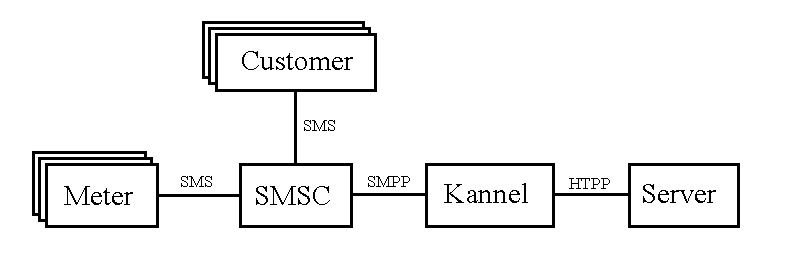
\includegraphics[width=\columnwidth]{figures/NetworkDiagram.pdf}
\end{center}
\caption{Network.}
\label{SoftwareDiagram}
\end{figure}


\begin{figure}[]
\begin{center}
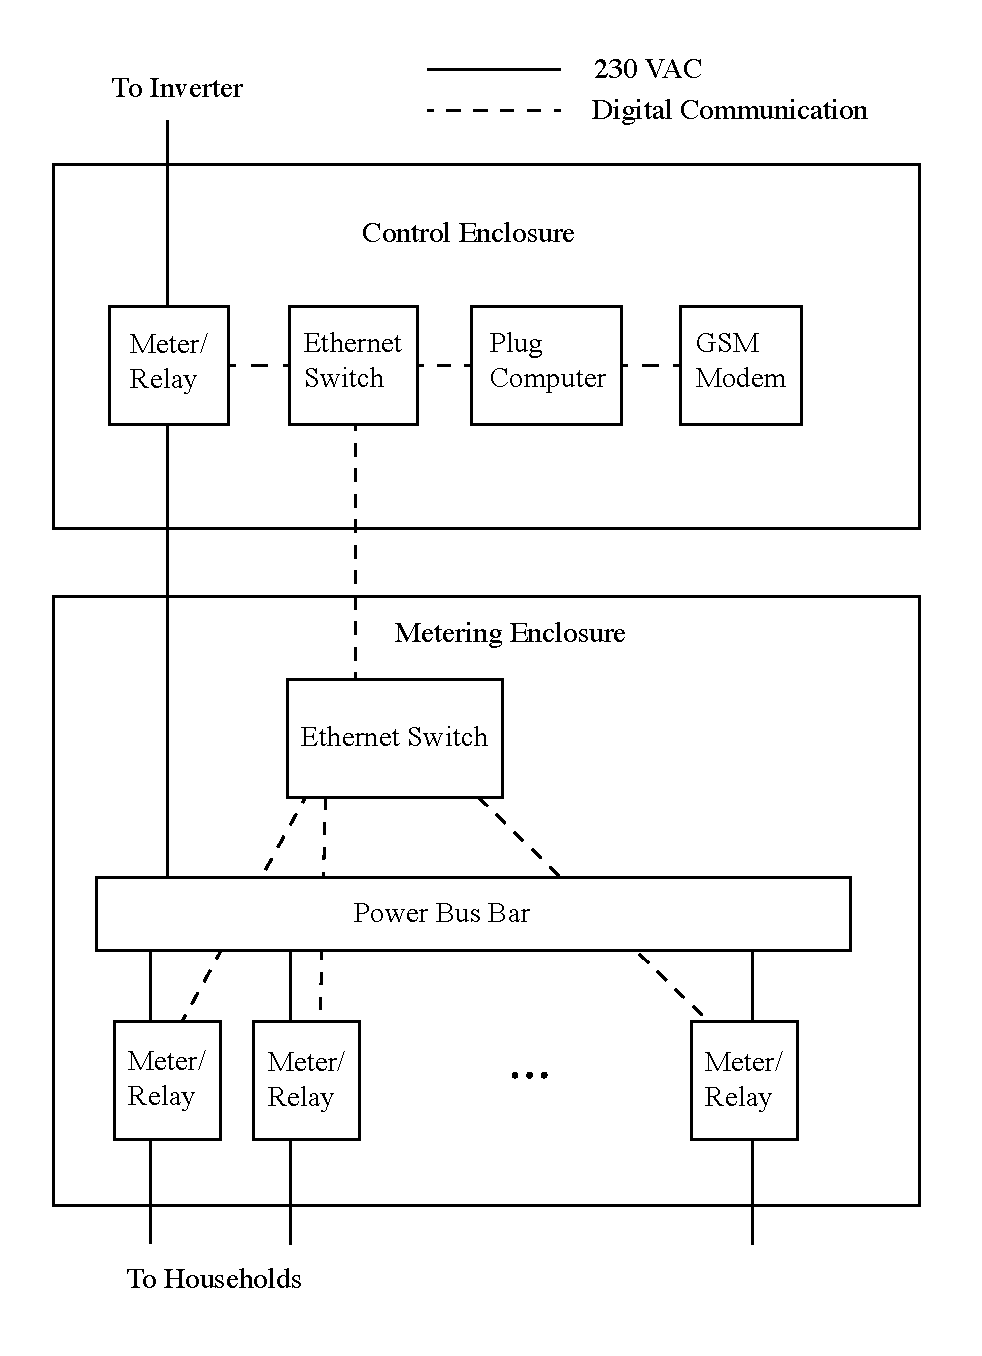
\includegraphics[width=\columnwidth]{figures/Enclosure.pdf}
\end{center}
\caption{Enclosure.}
\label{Enclosure}
\end{figure}


\begin{figure}[]
\begin{center}
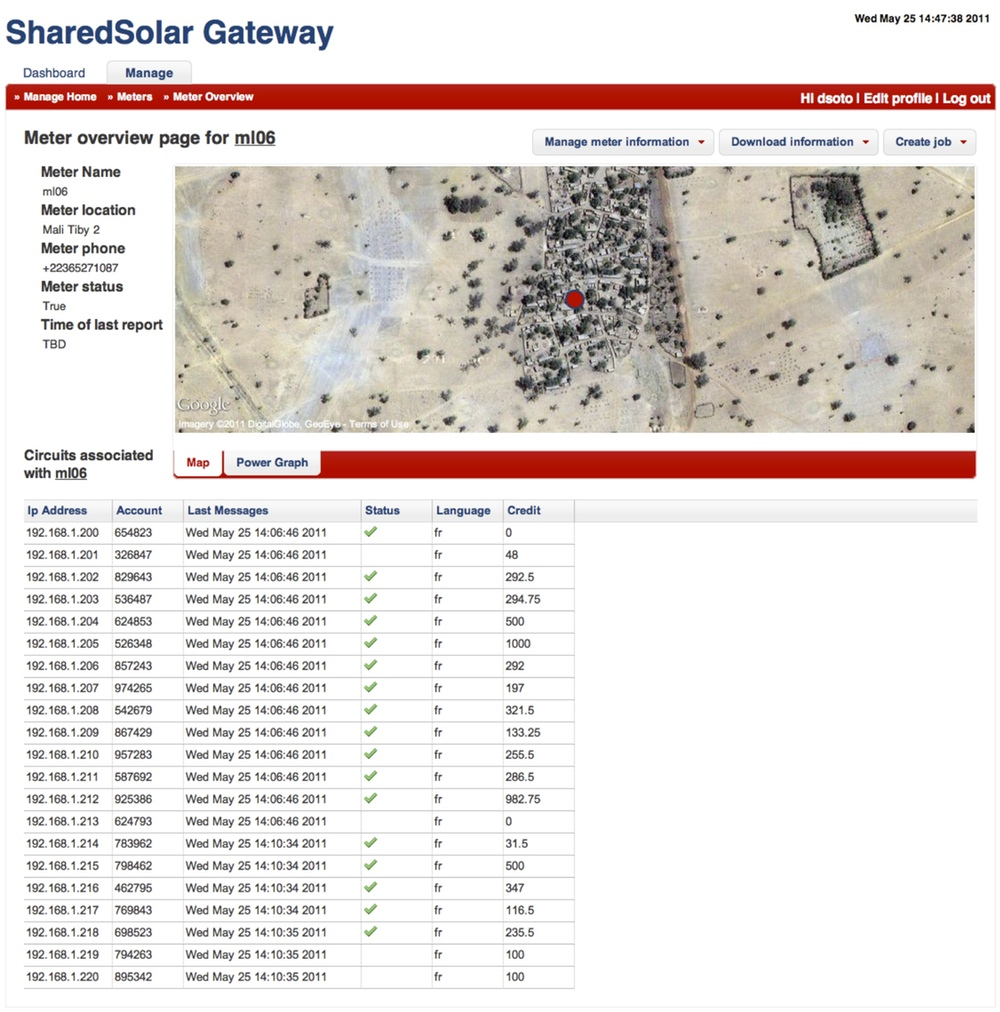
\includegraphics[width=\columnwidth]{figures/gateway.pdf}
\end{center}
\caption{Gateway.}
\label{gateway}
\end{figure}

\begin{figure}[]
\begin{center}
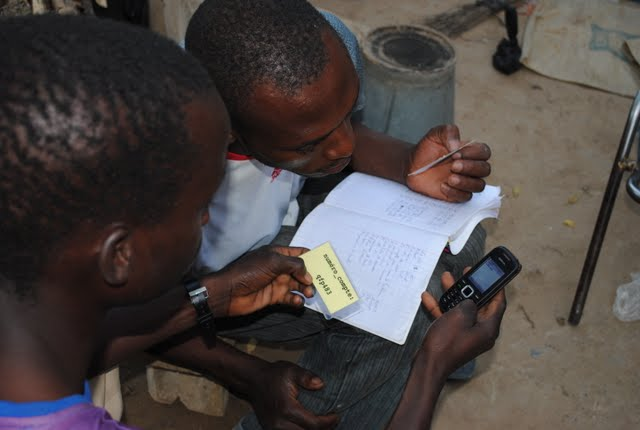
\includegraphics[width=\columnwidth]{figures/training.jpg}
\end{center}
\caption{Training.}
\label{training}
\end{figure}

\begin{figure}[]
\begin{center}
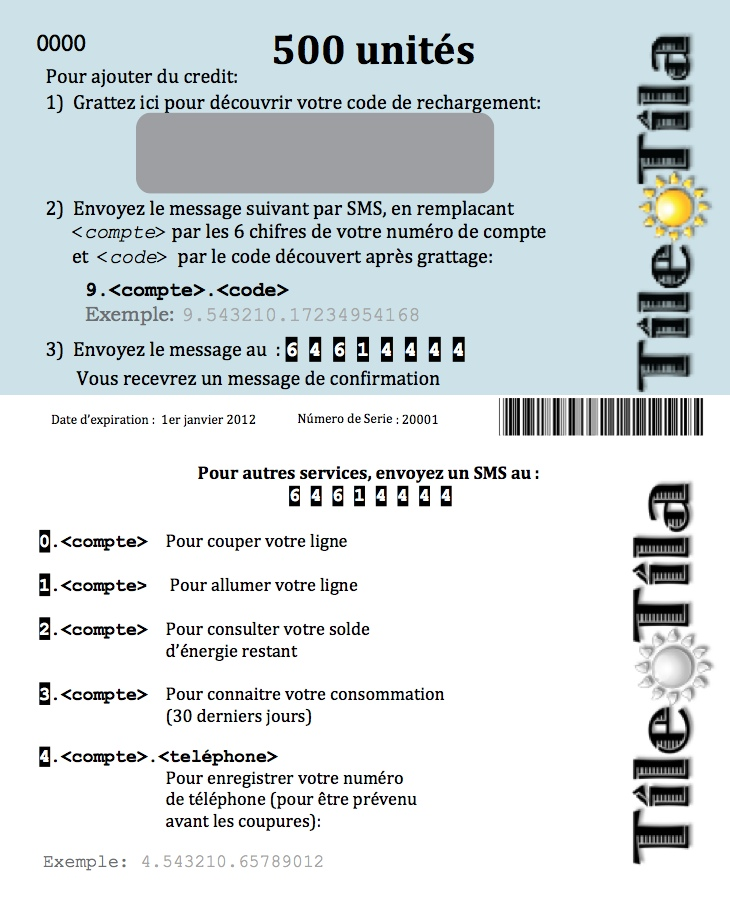
\includegraphics[width=\columnwidth]{figures/scratchCards.jpg}
\end{center}
\caption{Scratch cards.}
\label{scratchCards}
\end{figure}

\begin{figure}[]
\begin{center}
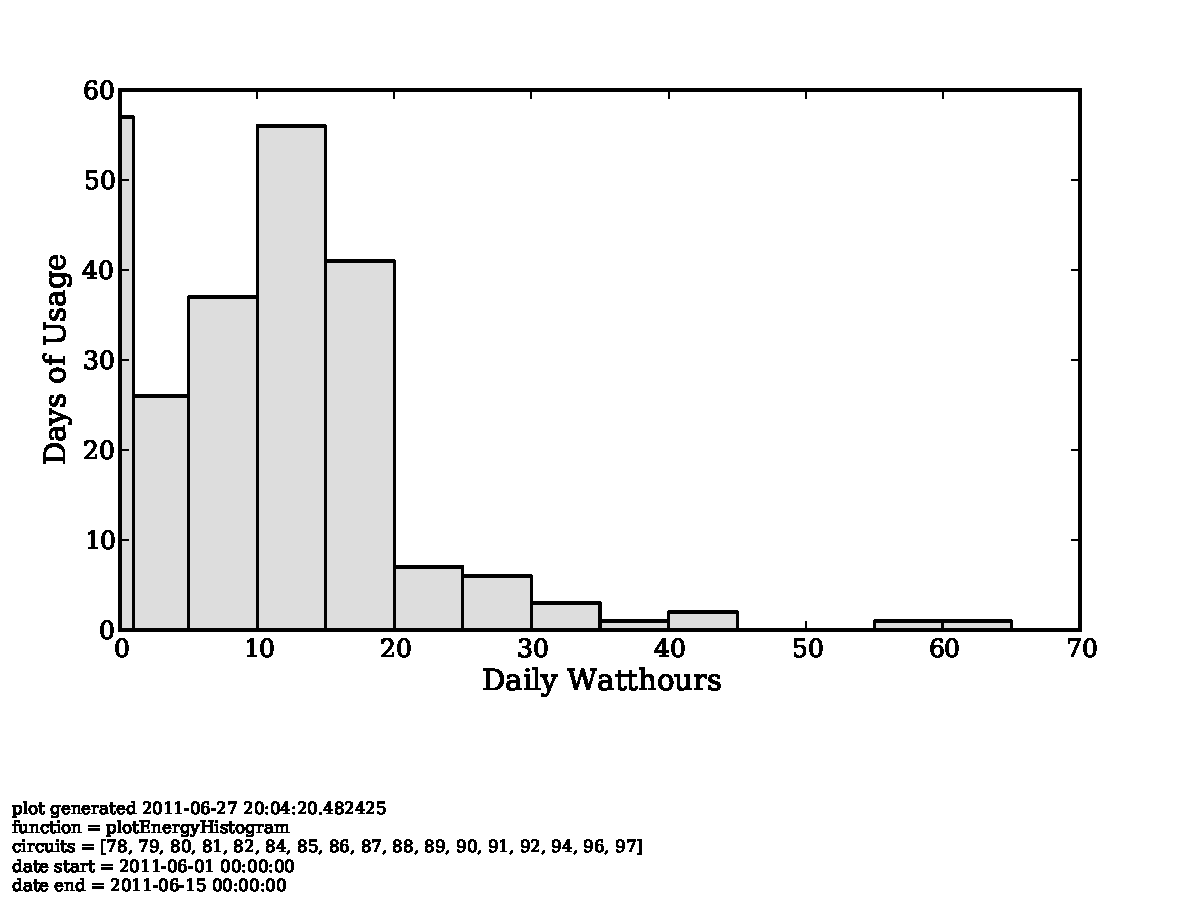
\includegraphics[width=\columnwidth]{figures/ml06Histogram.pdf}
\end{center}
\caption{Histogram of daily usage}
\label{ml06Histogram}
\end{figure}

\begin{figure}[]
\begin{center}
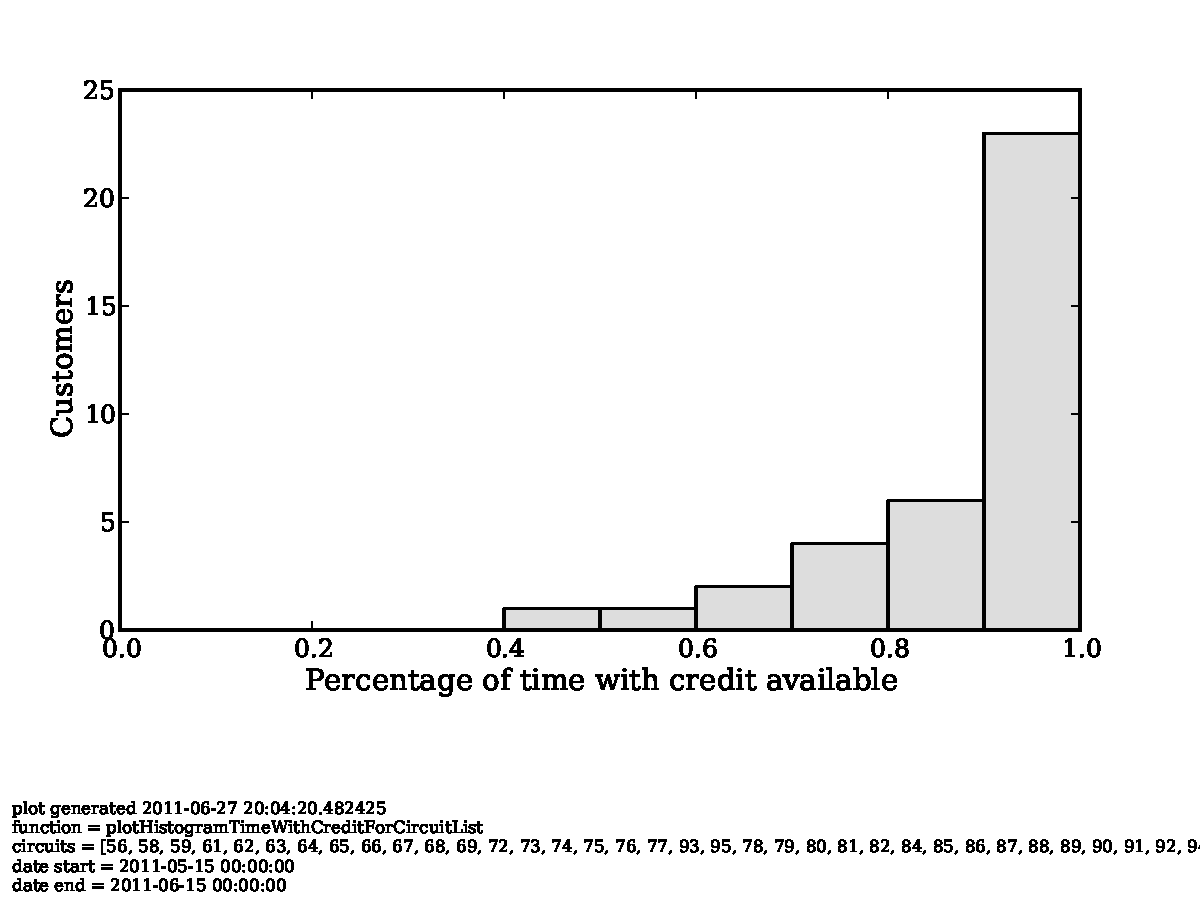
\includegraphics[width=\columnwidth]{figures/creditHistogram.pdf}
\end{center}
\caption{Histogram of percentage of time customers have available credit.}
\label{creditHistogram}
\end{figure}



\bibliography{architecture}
\bibliographystyle{plain}


\end{document}
